% Generated LaTeX file for compound CID: 536435
\documentclass[tikz]{standalone}
\definecolor{274A4A}{HTML}{274A4A}
\definecolor{FF0000}{HTML}{FF0000}
\begin{document}
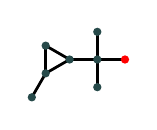
\begin{tikzpicture}[x=1pt,y=1pt]
  \draw[line width=1pt] (53.66,1.83) -- (43.66,1.83);
  \draw[line width=1pt] (33.66,1.83) -- (25.00,6.83);
  \draw[line width=1pt] (33.66,1.83) -- (43.66,1.83);
  \draw[line width=1pt] (33.66,1.83) -- (25.00,-3.17);
  \draw[line width=1pt] (25.00,6.83) -- (25.00,-3.17);
  \draw[line width=1pt] (43.66,1.83) -- (43.66,11.83);
  \draw[line width=1pt] (43.66,1.83) -- (43.66,-8.17);
  \draw[line width=1pt] (25.00,-3.17) -- (20.00,-11.83);
  \filldraw[fill=FF0000, draw=none] (53.66,1.83) circle (1.5pt);
  \filldraw[fill=274A4A, draw=none] (33.66,1.83) circle (1.5pt);
  \filldraw[fill=274A4A, draw=none] (25.00,6.83) circle (1.5pt);
  \filldraw[fill=274A4A, draw=none] (43.66,1.83) circle (1.5pt);
  \filldraw[fill=274A4A, draw=none] (25.00,-3.17) circle (1.5pt);
  \filldraw[fill=274A4A, draw=none] (43.66,11.83) circle (1.5pt);
  \filldraw[fill=274A4A, draw=none] (43.66,-8.17) circle (1.5pt);
  \filldraw[fill=274A4A, draw=none] (20.00,-11.83) circle (1.5pt);
\end{tikzpicture}
\end{document}